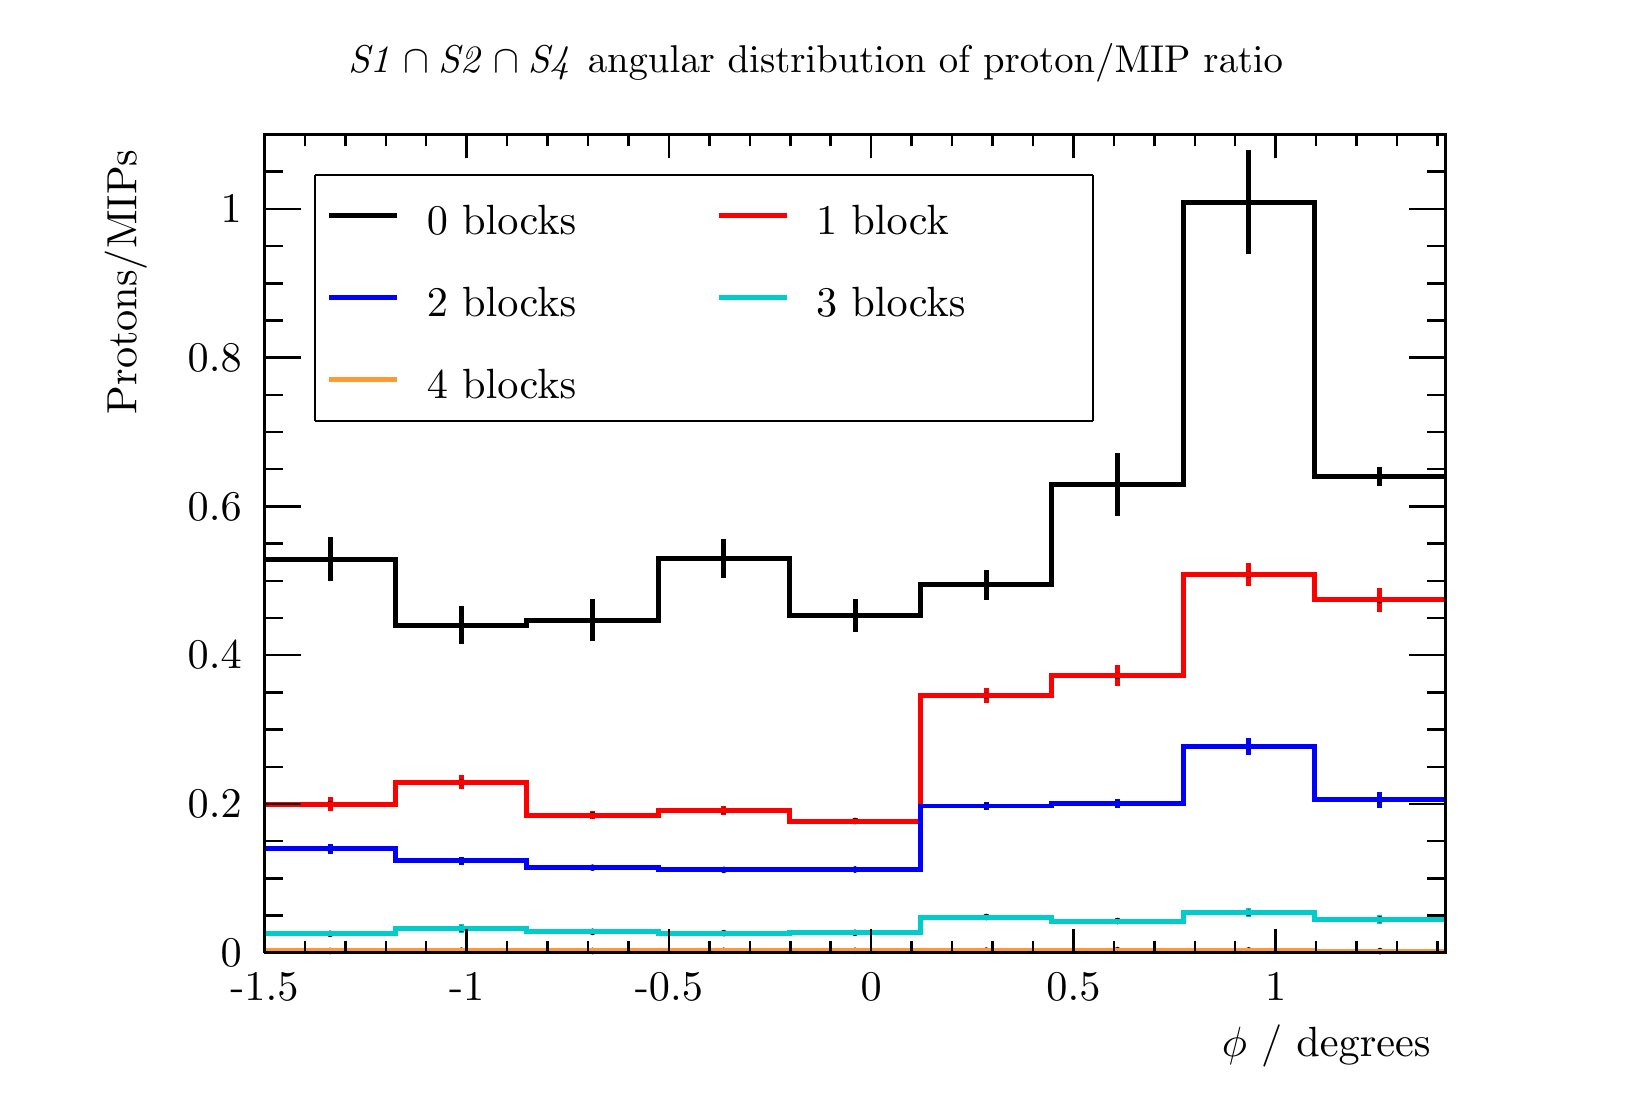
\begin{tikzpicture}
\pgfdeclareplotmark{cross} {
\pgfpathmoveto{\pgfpoint{-0.3\pgfplotmarksize}{\pgfplotmarksize}}
\pgfpathlineto{\pgfpoint{+0.3\pgfplotmarksize}{\pgfplotmarksize}}
\pgfpathlineto{\pgfpoint{+0.3\pgfplotmarksize}{0.3\pgfplotmarksize}}
\pgfpathlineto{\pgfpoint{+1\pgfplotmarksize}{0.3\pgfplotmarksize}}
\pgfpathlineto{\pgfpoint{+1\pgfplotmarksize}{-0.3\pgfplotmarksize}}
\pgfpathlineto{\pgfpoint{+0.3\pgfplotmarksize}{-0.3\pgfplotmarksize}}
\pgfpathlineto{\pgfpoint{+0.3\pgfplotmarksize}{-1.\pgfplotmarksize}}
\pgfpathlineto{\pgfpoint{-0.3\pgfplotmarksize}{-1.\pgfplotmarksize}}
\pgfpathlineto{\pgfpoint{-0.3\pgfplotmarksize}{-0.3\pgfplotmarksize}}
\pgfpathlineto{\pgfpoint{-1.\pgfplotmarksize}{-0.3\pgfplotmarksize}}
\pgfpathlineto{\pgfpoint{-1.\pgfplotmarksize}{0.3\pgfplotmarksize}}
\pgfpathlineto{\pgfpoint{-0.3\pgfplotmarksize}{0.3\pgfplotmarksize}}
\pgfpathclose
\pgfusepathqstroke
}
\pgfdeclareplotmark{cross*} {
\pgfpathmoveto{\pgfpoint{-0.3\pgfplotmarksize}{\pgfplotmarksize}}
\pgfpathlineto{\pgfpoint{+0.3\pgfplotmarksize}{\pgfplotmarksize}}
\pgfpathlineto{\pgfpoint{+0.3\pgfplotmarksize}{0.3\pgfplotmarksize}}
\pgfpathlineto{\pgfpoint{+1\pgfplotmarksize}{0.3\pgfplotmarksize}}
\pgfpathlineto{\pgfpoint{+1\pgfplotmarksize}{-0.3\pgfplotmarksize}}
\pgfpathlineto{\pgfpoint{+0.3\pgfplotmarksize}{-0.3\pgfplotmarksize}}
\pgfpathlineto{\pgfpoint{+0.3\pgfplotmarksize}{-1.\pgfplotmarksize}}
\pgfpathlineto{\pgfpoint{-0.3\pgfplotmarksize}{-1.\pgfplotmarksize}}
\pgfpathlineto{\pgfpoint{-0.3\pgfplotmarksize}{-0.3\pgfplotmarksize}}
\pgfpathlineto{\pgfpoint{-1.\pgfplotmarksize}{-0.3\pgfplotmarksize}}
\pgfpathlineto{\pgfpoint{-1.\pgfplotmarksize}{0.3\pgfplotmarksize}}
\pgfpathlineto{\pgfpoint{-0.3\pgfplotmarksize}{0.3\pgfplotmarksize}}
\pgfpathclose
\pgfusepathqfillstroke
}
\pgfdeclareplotmark{newstar} {
\pgfpathmoveto{\pgfqpoint{0pt}{\pgfplotmarksize}}
\pgfpathlineto{\pgfqpointpolar{44}{0.5\pgfplotmarksize}}
\pgfpathlineto{\pgfqpointpolar{18}{\pgfplotmarksize}}
\pgfpathlineto{\pgfqpointpolar{-20}{0.5\pgfplotmarksize}}
\pgfpathlineto{\pgfqpointpolar{-54}{\pgfplotmarksize}}
\pgfpathlineto{\pgfqpointpolar{-90}{0.5\pgfplotmarksize}}
\pgfpathlineto{\pgfqpointpolar{234}{\pgfplotmarksize}}
\pgfpathlineto{\pgfqpointpolar{198}{0.5\pgfplotmarksize}}
\pgfpathlineto{\pgfqpointpolar{162}{\pgfplotmarksize}}
\pgfpathlineto{\pgfqpointpolar{134}{0.5\pgfplotmarksize}}
\pgfpathclose
\pgfusepathqstroke
}
\pgfdeclareplotmark{newstar*} {
\pgfpathmoveto{\pgfqpoint{0pt}{\pgfplotmarksize}}
\pgfpathlineto{\pgfqpointpolar{44}{0.5\pgfplotmarksize}}
\pgfpathlineto{\pgfqpointpolar{18}{\pgfplotmarksize}}
\pgfpathlineto{\pgfqpointpolar{-20}{0.5\pgfplotmarksize}}
\pgfpathlineto{\pgfqpointpolar{-54}{\pgfplotmarksize}}
\pgfpathlineto{\pgfqpointpolar{-90}{0.5\pgfplotmarksize}}
\pgfpathlineto{\pgfqpointpolar{234}{\pgfplotmarksize}}
\pgfpathlineto{\pgfqpointpolar{198}{0.5\pgfplotmarksize}}
\pgfpathlineto{\pgfqpointpolar{162}{\pgfplotmarksize}}
\pgfpathlineto{\pgfqpointpolar{134}{0.5\pgfplotmarksize}}
\pgfpathclose
\pgfusepathqfillstroke
}
\definecolor{c}{rgb}{1,1,1};
\draw [color=c, fill=c] (0,0) rectangle (20,13.4957);
\draw [color=c, fill=c] (3,1.75444) rectangle (18,12.1461);
\definecolor{c}{rgb}{0,0,0};
\draw [c,line width=0.9] (3,1.75444) -- (3,12.1461) -- (18,12.1461) -- (18,1.75444) -- (3,1.75444);
\definecolor{c}{rgb}{1,1,1};
\draw [color=c, fill=c] (3,1.75444) rectangle (18,12.1461);
\definecolor{c}{rgb}{0,0,0};
\draw [c,line width=0.9] (3,1.75444) -- (3,12.1461) -- (18,12.1461) -- (18,1.75444) -- (3,1.75444);
\draw [c,line width=0.9] (3,1.75444) -- (4.66667,1.75444) -- (4.66667,1.75444) -- (6.33333,1.75444) -- (6.33333,1.75444) -- (8,1.75444) -- (8,1.75444) -- (9.66667,1.75444) -- (9.66667,1.75444) -- (11.3333,1.75444) -- (11.3333,1.75444) -- (13,1.75444)
 -- (13,1.75444) -- (14.6667,1.75444) -- (14.6667,1.75444) -- (16.3333,1.75444) -- (16.3333,1.75444) -- (18,1.75444);
\draw [c,line width=0.9] (3,1.75444) -- (18,1.75444);
\draw [c,line width=0.9] (3,2.05809) -- (3,1.75444);
\draw [c,line width=0.9] (3.5137,1.90627) -- (3.5137,1.75444);
\draw [c,line width=0.9] (4.0274,1.90627) -- (4.0274,1.75444);
\draw [c,line width=0.9] (4.5411,1.90627) -- (4.5411,1.75444);
\draw [c,line width=0.9] (5.05479,1.90627) -- (5.05479,1.75444);
\draw [c,line width=0.9] (5.56849,2.05809) -- (5.56849,1.75444);
\draw [c,line width=0.9] (6.08219,1.90627) -- (6.08219,1.75444);
\draw [c,line width=0.9] (6.59589,1.90627) -- (6.59589,1.75444);
\draw [c,line width=0.9] (7.10959,1.90627) -- (7.10959,1.75444);
\draw [c,line width=0.9] (7.62329,1.90627) -- (7.62329,1.75444);
\draw [c,line width=0.9] (8.13699,2.05809) -- (8.13699,1.75444);
\draw [c,line width=0.9] (8.65069,1.90627) -- (8.65069,1.75444);
\draw [c,line width=0.9] (9.16438,1.90627) -- (9.16438,1.75444);
\draw [c,line width=0.9] (9.67808,1.90627) -- (9.67808,1.75444);
\draw [c,line width=0.9] (10.1918,1.90627) -- (10.1918,1.75444);
\draw [c,line width=0.9] (10.7055,2.05809) -- (10.7055,1.75444);
\draw [c,line width=0.9] (11.2192,1.90627) -- (11.2192,1.75444);
\draw [c,line width=0.9] (11.7329,1.90627) -- (11.7329,1.75444);
\draw [c,line width=0.9] (12.2466,1.90627) -- (12.2466,1.75444);
\draw [c,line width=0.9] (12.7603,1.90627) -- (12.7603,1.75444);
\draw [c,line width=0.9] (13.274,2.05809) -- (13.274,1.75444);
\draw [c,line width=0.9] (13.7877,1.90627) -- (13.7877,1.75444);
\draw [c,line width=0.9] (14.3014,1.90627) -- (14.3014,1.75444);
\draw [c,line width=0.9] (14.8151,1.90627) -- (14.8151,1.75444);
\draw [c,line width=0.9] (15.3288,1.90627) -- (15.3288,1.75444);
\draw [c,line width=0.9] (15.8425,2.05809) -- (15.8425,1.75444);
\draw [c,line width=0.9] (15.8425,2.05809) -- (15.8425,1.75444);
\draw [c,line width=0.9] (16.3562,1.90627) -- (16.3562,1.75444);
\draw [c,line width=0.9] (16.8699,1.90627) -- (16.8699,1.75444);
\draw [c,line width=0.9] (17.3836,1.90627) -- (17.3836,1.75444);
\draw [c,line width=0.9] (17.8973,1.90627) -- (17.8973,1.75444);
\draw [anchor=base] (3,1.14713) node[scale=1.52731, color=c, rotate=0]{-1.5};
\draw [anchor=base] (5.56849,1.14713) node[scale=1.52731, color=c, rotate=0]{-1};
\draw [anchor=base] (8.13699,1.14713) node[scale=1.52731, color=c, rotate=0]{-0.5};
\draw [anchor=base] (10.7055,1.14713) node[scale=1.52731, color=c, rotate=0]{0};
\draw [anchor=base] (13.274,1.14713) node[scale=1.52731, color=c, rotate=0]{0.5};
\draw [anchor=base] (15.8425,1.14713) node[scale=1.52731, color=c, rotate=0]{1};
\draw [anchor= east] (18,0.566819) node[scale=1.52731, color=c, rotate=0]{$ \phi$ / degrees};
\draw [c,line width=0.9] (3,12.1461) -- (18,12.1461);
\draw [c,line width=0.9] (3,11.8425) -- (3,12.1461);
\draw [c,line width=0.9] (3.5137,11.9943) -- (3.5137,12.1461);
\draw [c,line width=0.9] (4.0274,11.9943) -- (4.0274,12.1461);
\draw [c,line width=0.9] (4.5411,11.9943) -- (4.5411,12.1461);
\draw [c,line width=0.9] (5.05479,11.9943) -- (5.05479,12.1461);
\draw [c,line width=0.9] (5.56849,11.8425) -- (5.56849,12.1461);
\draw [c,line width=0.9] (6.08219,11.9943) -- (6.08219,12.1461);
\draw [c,line width=0.9] (6.59589,11.9943) -- (6.59589,12.1461);
\draw [c,line width=0.9] (7.10959,11.9943) -- (7.10959,12.1461);
\draw [c,line width=0.9] (7.62329,11.9943) -- (7.62329,12.1461);
\draw [c,line width=0.9] (8.13699,11.8425) -- (8.13699,12.1461);
\draw [c,line width=0.9] (8.65069,11.9943) -- (8.65069,12.1461);
\draw [c,line width=0.9] (9.16438,11.9943) -- (9.16438,12.1461);
\draw [c,line width=0.9] (9.67808,11.9943) -- (9.67808,12.1461);
\draw [c,line width=0.9] (10.1918,11.9943) -- (10.1918,12.1461);
\draw [c,line width=0.9] (10.7055,11.8425) -- (10.7055,12.1461);
\draw [c,line width=0.9] (11.2192,11.9943) -- (11.2192,12.1461);
\draw [c,line width=0.9] (11.7329,11.9943) -- (11.7329,12.1461);
\draw [c,line width=0.9] (12.2466,11.9943) -- (12.2466,12.1461);
\draw [c,line width=0.9] (12.7603,11.9943) -- (12.7603,12.1461);
\draw [c,line width=0.9] (13.274,11.8425) -- (13.274,12.1461);
\draw [c,line width=0.9] (13.7877,11.9943) -- (13.7877,12.1461);
\draw [c,line width=0.9] (14.3014,11.9943) -- (14.3014,12.1461);
\draw [c,line width=0.9] (14.8151,11.9943) -- (14.8151,12.1461);
\draw [c,line width=0.9] (15.3288,11.9943) -- (15.3288,12.1461);
\draw [c,line width=0.9] (15.8425,11.8425) -- (15.8425,12.1461);
\draw [c,line width=0.9] (15.8425,11.8425) -- (15.8425,12.1461);
\draw [c,line width=0.9] (16.3562,11.9943) -- (16.3562,12.1461);
\draw [c,line width=0.9] (16.8699,11.9943) -- (16.8699,12.1461);
\draw [c,line width=0.9] (17.3836,11.9943) -- (17.3836,12.1461);
\draw [c,line width=0.9] (17.8973,11.9943) -- (17.8973,12.1461);
\draw [c,line width=0.9] (3,1.75444) -- (3,12.1461);
\draw [c,line width=0.9] (3.462,1.75444) -- (3,1.75444);
\draw [c,line width=0.9] (3.231,2.22679) -- (3,2.22679);
\draw [c,line width=0.9] (3.231,2.69914) -- (3,2.69914);
\draw [c,line width=0.9] (3.231,3.17149) -- (3,3.17149);
\draw [c,line width=0.9] (3.462,3.64384) -- (3,3.64384);
\draw [c,line width=0.9] (3.231,4.11619) -- (3,4.11619);
\draw [c,line width=0.9] (3.231,4.58854) -- (3,4.58854);
\draw [c,line width=0.9] (3.231,5.06089) -- (3,5.06089);
\draw [c,line width=0.9] (3.462,5.53324) -- (3,5.53324);
\draw [c,line width=0.9] (3.231,6.00559) -- (3,6.00559);
\draw [c,line width=0.9] (3.231,6.47794) -- (3,6.47794);
\draw [c,line width=0.9] (3.231,6.95029) -- (3,6.95029);
\draw [c,line width=0.9] (3.462,7.42264) -- (3,7.42264);
\draw [c,line width=0.9] (3.231,7.89499) -- (3,7.89499);
\draw [c,line width=0.9] (3.231,8.36734) -- (3,8.36734);
\draw [c,line width=0.9] (3.231,8.83968) -- (3,8.83968);
\draw [c,line width=0.9] (3.462,9.31203) -- (3,9.31203);
\draw [c,line width=0.9] (3.231,9.78438) -- (3,9.78438);
\draw [c,line width=0.9] (3.231,10.2567) -- (3,10.2567);
\draw [c,line width=0.9] (3.231,10.7291) -- (3,10.7291);
\draw [c,line width=0.9] (3.462,11.2014) -- (3,11.2014);
\draw [c,line width=0.9] (3.462,11.2014) -- (3,11.2014);
\draw [c,line width=0.9] (3.231,11.6738) -- (3,11.6738);
\draw [c,line width=0.9] (3.231,12.1461) -- (3,12.1461);
\draw [anchor= east] (2.9,1.75444) node[scale=1.52731, color=c, rotate=0]{0};
\draw [anchor= east] (2.9,3.64384) node[scale=1.52731, color=c, rotate=0]{0.2};
\draw [anchor= east] (2.9,5.53324) node[scale=1.52731, color=c, rotate=0]{0.4};
\draw [anchor= east] (2.9,7.42264) node[scale=1.52731, color=c, rotate=0]{0.6};
\draw [anchor= east] (2.9,9.31203) node[scale=1.52731, color=c, rotate=0]{0.8};
\draw [anchor= east] (2.9,11.2014) node[scale=1.52731, color=c, rotate=0]{1};
\draw [anchor= east] (1.24,12.1461) node[scale=1.52731, color=c, rotate=90]{ Protons/MIPs};
\draw [c,line width=0.9] (18,1.75444) -- (18,12.1461);
\draw [c,line width=0.9] (17.538,1.75444) -- (18,1.75444);
\draw [c,line width=0.9] (17.769,2.22679) -- (18,2.22679);
\draw [c,line width=0.9] (17.769,2.69914) -- (18,2.69914);
\draw [c,line width=0.9] (17.769,3.17149) -- (18,3.17149);
\draw [c,line width=0.9] (17.538,3.64384) -- (18,3.64384);
\draw [c,line width=0.9] (17.769,4.11619) -- (18,4.11619);
\draw [c,line width=0.9] (17.769,4.58854) -- (18,4.58854);
\draw [c,line width=0.9] (17.769,5.06089) -- (18,5.06089);
\draw [c,line width=0.9] (17.538,5.53324) -- (18,5.53324);
\draw [c,line width=0.9] (17.769,6.00559) -- (18,6.00559);
\draw [c,line width=0.9] (17.769,6.47794) -- (18,6.47794);
\draw [c,line width=0.9] (17.769,6.95029) -- (18,6.95029);
\draw [c,line width=0.9] (17.538,7.42264) -- (18,7.42264);
\draw [c,line width=0.9] (17.769,7.89499) -- (18,7.89499);
\draw [c,line width=0.9] (17.769,8.36734) -- (18,8.36734);
\draw [c,line width=0.9] (17.769,8.83968) -- (18,8.83968);
\draw [c,line width=0.9] (17.538,9.31203) -- (18,9.31203);
\draw [c,line width=0.9] (17.769,9.78438) -- (18,9.78438);
\draw [c,line width=0.9] (17.769,10.2567) -- (18,10.2567);
\draw [c,line width=0.9] (17.769,10.7291) -- (18,10.7291);
\draw [c,line width=0.9] (17.538,11.2014) -- (18,11.2014);
\draw [c,line width=0.9] (17.538,11.2014) -- (18,11.2014);
\draw [c,line width=0.9] (17.769,11.6738) -- (18,11.6738);
\draw [c,line width=0.9] (17.769,12.1461) -- (18,12.1461);
\draw [c,line width=1.8] (3.83333,6.47098) -- (3.83333,6.75147);
\draw [c,line width=1.8] (3.83333,6.75147) -- (3.83333,7.03195);
\foreach \P in {(3.83333,6.75147)}{\draw[mark options={color=c,fill=c},mark size=2.402402pt,mark=*,mark size=1pt] plot coordinates {\P};}
\draw [c,line width=1.8] (5.5,5.67509) -- (5.5,5.91461);
\draw [c,line width=1.8] (5.5,5.91461) -- (5.5,6.15413);
\foreach \P in {(5.5,5.91461)}{\draw[mark options={color=c,fill=c},mark size=2.402402pt,mark=*,mark size=1pt] plot coordinates {\P};}
\draw [c,line width=1.8] (7.16667,5.7124) -- (7.16667,5.97841);
\draw [c,line width=1.8] (7.16667,5.97841) -- (7.16667,6.24442);
\foreach \P in {(7.16667,5.97841)}{\draw[mark options={color=c,fill=c},mark size=2.402402pt,mark=*,mark size=1pt] plot coordinates {\P};}
\draw [c,line width=1.8] (8.83333,6.5106) -- (8.83333,6.761);
\draw [c,line width=1.8] (8.83333,6.761) -- (8.83333,7.01141);
\foreach \P in {(8.83333,6.761)}{\draw[mark options={color=c,fill=c},mark size=2.402402pt,mark=*,mark size=1pt] plot coordinates {\P};}
\draw [c,line width=1.8] (10.5,5.83134) -- (10.5,6.03742);
\draw [c,line width=1.8] (10.5,6.03742) -- (10.5,6.2435);
\foreach \P in {(10.5,6.03742)}{\draw[mark options={color=c,fill=c},mark size=2.402402pt,mark=*,mark size=1pt] plot coordinates {\P};}
\draw [c,line width=1.8] (12.1667,6.23357) -- (12.1667,6.42605);
\draw [c,line width=1.8] (12.1667,6.42605) -- (12.1667,6.61853);
\foreach \P in {(12.1667,6.42605)}{\draw[mark options={color=c,fill=c},mark size=2.402402pt,mark=*,mark size=1pt] plot coordinates {\P};}
\draw [c,line width=1.8] (13.8333,7.30043) -- (13.8333,7.70355);
\draw [c,line width=1.8] (13.8333,7.70355) -- (13.8333,8.10667);
\foreach \P in {(13.8333,7.70355)}{\draw[mark options={color=c,fill=c},mark size=2.402402pt,mark=*,mark size=1pt] plot coordinates {\P};}
\draw [c,line width=1.8] (15.5,10.6281) -- (15.5,11.2872);
\draw [c,line width=1.8] (15.5,11.2872) -- (15.5,11.9463);
\foreach \P in {(15.5,11.2872)}{\draw[mark options={color=c,fill=c},mark size=2.402402pt,mark=*,mark size=1pt] plot coordinates {\P};}
\draw [c,line width=1.8] (17.1667,7.67629) -- (17.1667,7.8003);
\draw [c,line width=1.8] (17.1667,7.8003) -- (17.1667,7.9243);
\foreach \P in {(17.1667,7.8003)}{\draw[mark options={color=c,fill=c},mark size=2.402402pt,mark=*,mark size=1pt] plot coordinates {\P};}
\draw [c,line width=1.8] (3,6.75147) -- (4.66667,6.75147) -- (4.66667,5.91461) -- (6.33333,5.91461) -- (6.33333,5.97841) -- (8,5.97841) -- (8,6.761) -- (9.66667,6.761) -- (9.66667,6.03742) -- (11.3333,6.03742) -- (11.3333,6.42605) -- (13,6.42605) --
 (13,7.70355) -- (14.6667,7.70355) -- (14.6667,11.2872) -- (16.3333,11.2872) -- (16.3333,7.8003) -- (18,7.8003);
\definecolor{c}{rgb}{1,0,0};
\draw [c,line width=1.8] (3.83333,3.5515) -- (3.83333,3.64187);
\draw [c,line width=1.8] (3.83333,3.64187) -- (3.83333,3.73225);
\definecolor{c}{rgb}{0,0,0};
\foreach \P in {(3.83333,3.64187)}{\draw[mark options={color=c,fill=c},mark size=2.402402pt,mark=*,mark size=1pt] plot coordinates {\P};}
\definecolor{c}{rgb}{1,0,0};
\draw [c,line width=1.8] (5.5,3.83082) -- (5.5,3.91831);
\draw [c,line width=1.8] (5.5,3.91831) -- (5.5,4.00579);
\definecolor{c}{rgb}{0,0,0};
\foreach \P in {(5.5,3.91831)}{\draw[mark options={color=c,fill=c},mark size=2.402402pt,mark=*,mark size=1pt] plot coordinates {\P};}
\definecolor{c}{rgb}{1,0,0};
\draw [c,line width=1.8] (7.16667,3.45285) -- (7.16667,3.50294);
\draw [c,line width=1.8] (7.16667,3.50294) -- (7.16667,3.55304);
\definecolor{c}{rgb}{0,0,0};
\foreach \P in {(7.16667,3.50294)}{\draw[mark options={color=c,fill=c},mark size=2.402402pt,mark=*,mark size=1pt] plot coordinates {\P};}
\definecolor{c}{rgb}{1,0,0};
\draw [c,line width=1.8] (8.83333,3.50273) -- (8.83333,3.55771);
\draw [c,line width=1.8] (8.83333,3.55771) -- (8.83333,3.61269);
\definecolor{c}{rgb}{0,0,0};
\foreach \P in {(8.83333,3.55771)}{\draw[mark options={color=c,fill=c},mark size=2.402402pt,mark=*,mark size=1pt] plot coordinates {\P};}
\definecolor{c}{rgb}{1,0,0};
\draw [c,line width=1.8] (10.5,3.38392) -- (10.5,3.4271);
\draw [c,line width=1.8] (10.5,3.4271) -- (10.5,3.47028);
\definecolor{c}{rgb}{0,0,0};
\foreach \P in {(10.5,3.4271)}{\draw[mark options={color=c,fill=c},mark size=2.402402pt,mark=*,mark size=1pt] plot coordinates {\P};}
\definecolor{c}{rgb}{1,0,0};
\draw [c,line width=1.8] (12.1667,4.92863) -- (12.1667,5.01975);
\draw [c,line width=1.8] (12.1667,5.01975) -- (12.1667,5.11087);
\definecolor{c}{rgb}{0,0,0};
\foreach \P in {(12.1667,5.01975)}{\draw[mark options={color=c,fill=c},mark size=2.402402pt,mark=*,mark size=1pt] plot coordinates {\P};}
\definecolor{c}{rgb}{1,0,0};
\draw [c,line width=1.8] (13.8333,5.13804) -- (13.8333,5.2703);
\draw [c,line width=1.8] (13.8333,5.2703) -- (13.8333,5.40255);
\definecolor{c}{rgb}{0,0,0};
\foreach \P in {(13.8333,5.2703)}{\draw[mark options={color=c,fill=c},mark size=2.402402pt,mark=*,mark size=1pt] plot coordinates {\P};}
\definecolor{c}{rgb}{1,0,0};
\draw [c,line width=1.8] (15.5,6.41063) -- (15.5,6.55525);
\draw [c,line width=1.8] (15.5,6.55525) -- (15.5,6.69987);
\definecolor{c}{rgb}{0,0,0};
\foreach \P in {(15.5,6.55525)}{\draw[mark options={color=c,fill=c},mark size=2.402402pt,mark=*,mark size=1pt] plot coordinates {\P};}
\definecolor{c}{rgb}{1,0,0};
\draw [c,line width=1.8] (17.1667,6.08006) -- (17.1667,6.23534);
\draw [c,line width=1.8] (17.1667,6.23534) -- (17.1667,6.39062);
\definecolor{c}{rgb}{0,0,0};
\foreach \P in {(17.1667,6.23534)}{\draw[mark options={color=c,fill=c},mark size=2.402402pt,mark=*,mark size=1pt] plot coordinates {\P};}
\definecolor{c}{rgb}{1,0,0};
\draw [c,line width=1.8] (3,3.64187) -- (4.66667,3.64187) -- (4.66667,3.91831) -- (6.33333,3.91831) -- (6.33333,3.50294) -- (8,3.50294) -- (8,3.55771) -- (9.66667,3.55771) -- (9.66667,3.4271) -- (11.3333,3.4271) -- (11.3333,5.01975) -- (13,5.01975)
 -- (13,5.2703) -- (14.6667,5.2703) -- (14.6667,6.55525) -- (16.3333,6.55525) -- (16.3333,6.23534) -- (18,6.23534);
\definecolor{c}{rgb}{0,0,1};
\draw [c,line width=1.8] (3.83333,3.01041) -- (3.83333,3.07368);
\draw [c,line width=1.8] (3.83333,3.07368) -- (3.83333,3.13695);
\definecolor{c}{rgb}{0,0,0};
\foreach \P in {(3.83333,3.07368)}{\draw[mark options={color=c,fill=c},mark size=2.402402pt,mark=*,mark size=1pt] plot coordinates {\P};}
\definecolor{c}{rgb}{0,0,1};
\draw [c,line width=1.8] (5.5,2.87371) -- (5.5,2.92322);
\draw [c,line width=1.8] (5.5,2.92322) -- (5.5,2.97274);
\definecolor{c}{rgb}{0,0,0};
\foreach \P in {(5.5,2.92322)}{\draw[mark options={color=c,fill=c},mark size=2.402402pt,mark=*,mark size=1pt] plot coordinates {\P};}
\definecolor{c}{rgb}{0,0,1};
\draw [c,line width=1.8] (7.16667,2.79978) -- (7.16667,2.83455);
\draw [c,line width=1.8] (7.16667,2.83455) -- (7.16667,2.86931);
\definecolor{c}{rgb}{0,0,0};
\foreach \P in {(7.16667,2.83455)}{\draw[mark options={color=c,fill=c},mark size=2.402402pt,mark=*,mark size=1pt] plot coordinates {\P};}
\definecolor{c}{rgb}{0,0,1};
\draw [c,line width=1.8] (8.83333,2.77705) -- (8.83333,2.80662);
\draw [c,line width=1.8] (8.83333,2.80662) -- (8.83333,2.83618);
\definecolor{c}{rgb}{0,0,0};
\foreach \P in {(8.83333,2.80662)}{\draw[mark options={color=c,fill=c},mark size=2.402402pt,mark=*,mark size=1pt] plot coordinates {\P};}
\definecolor{c}{rgb}{0,0,1};
\draw [c,line width=1.8] (10.5,2.78559) -- (10.5,2.8113);
\draw [c,line width=1.8] (10.5,2.8113) -- (10.5,2.83701);
\definecolor{c}{rgb}{0,0,0};
\foreach \P in {(10.5,2.8113)}{\draw[mark options={color=c,fill=c},mark size=2.402402pt,mark=*,mark size=1pt] plot coordinates {\P};}
\definecolor{c}{rgb}{0,0,1};
\draw [c,line width=1.8] (12.1667,3.56421) -- (12.1667,3.61803);
\draw [c,line width=1.8] (12.1667,3.61803) -- (12.1667,3.67185);
\definecolor{c}{rgb}{0,0,0};
\foreach \P in {(12.1667,3.61803)}{\draw[mark options={color=c,fill=c},mark size=2.402402pt,mark=*,mark size=1pt] plot coordinates {\P};}
\definecolor{c}{rgb}{0,0,1};
\draw [c,line width=1.8] (13.8333,3.59195) -- (13.8333,3.6503);
\draw [c,line width=1.8] (13.8333,3.6503) -- (13.8333,3.70864);
\definecolor{c}{rgb}{0,0,0};
\foreach \P in {(13.8333,3.6503)}{\draw[mark options={color=c,fill=c},mark size=2.402402pt,mark=*,mark size=1pt] plot coordinates {\P};}
\definecolor{c}{rgb}{0,0,1};
\draw [c,line width=1.8] (15.5,4.26456) -- (15.5,4.3705);
\draw [c,line width=1.8] (15.5,4.3705) -- (15.5,4.47644);
\definecolor{c}{rgb}{0,0,0};
\foreach \P in {(15.5,4.3705)}{\draw[mark options={color=c,fill=c},mark size=2.402402pt,mark=*,mark size=1pt] plot coordinates {\P};}
\definecolor{c}{rgb}{0,0,1};
\draw [c,line width=1.8] (17.1667,3.59621) -- (17.1667,3.69452);
\draw [c,line width=1.8] (17.1667,3.69452) -- (17.1667,3.79283);
\definecolor{c}{rgb}{0,0,0};
\foreach \P in {(17.1667,3.69452)}{\draw[mark options={color=c,fill=c},mark size=2.402402pt,mark=*,mark size=1pt] plot coordinates {\P};}
\definecolor{c}{rgb}{0,0,1};
\draw [c,line width=1.8] (3,3.07368) -- (4.66667,3.07368) -- (4.66667,2.92322) -- (6.33333,2.92322) -- (6.33333,2.83455) -- (8,2.83455) -- (8,2.80662) -- (9.66667,2.80662) -- (9.66667,2.8113) -- (11.3333,2.8113) -- (11.3333,3.61803) -- (13,3.61803)
 -- (13,3.6503) -- (14.6667,3.6503) -- (14.6667,4.3705) -- (16.3333,4.3705) -- (16.3333,3.69452) -- (18,3.69452);
\definecolor{c}{rgb}{0,0.8,0.8};
\draw [c,line width=1.8] (3.83333,1.96496) -- (3.83333,1.99447);
\draw [c,line width=1.8] (3.83333,1.99447) -- (3.83333,2.02397);
\definecolor{c}{rgb}{0,0,0};
\foreach \P in {(3.83333,1.99447)}{\draw[mark options={color=c,fill=c},mark size=2.402402pt,mark=*,mark size=1pt] plot coordinates {\P};}
\definecolor{c}{rgb}{0,0.8,0.8};
\draw [c,line width=1.8] (5.5,2.00196) -- (5.5,2.05849);
\draw [c,line width=1.8] (5.5,2.05849) -- (5.5,2.11501);
\definecolor{c}{rgb}{0,0,0};
\foreach \P in {(5.5,2.05849)}{\draw[mark options={color=c,fill=c},mark size=2.402402pt,mark=*,mark size=1pt] plot coordinates {\P};}
\definecolor{c}{rgb}{0,0.8,0.8};
\draw [c,line width=1.8] (7.16667,1.9969) -- (7.16667,2.02031);
\draw [c,line width=1.8] (7.16667,2.02031) -- (7.16667,2.04371);
\definecolor{c}{rgb}{0,0,0};
\foreach \P in {(7.16667,2.02031)}{\draw[mark options={color=c,fill=c},mark size=2.402402pt,mark=*,mark size=1pt] plot coordinates {\P};}
\definecolor{c}{rgb}{0,0.8,0.8};
\draw [c,line width=1.8] (8.83333,1.98128) -- (8.83333,2.00355);
\draw [c,line width=1.8] (8.83333,2.00355) -- (8.83333,2.02582);
\definecolor{c}{rgb}{0,0,0};
\foreach \P in {(8.83333,2.00355)}{\draw[mark options={color=c,fill=c},mark size=2.402402pt,mark=*,mark size=1pt] plot coordinates {\P};}
\definecolor{c}{rgb}{0,0.8,0.8};
\draw [c,line width=1.8] (10.5,1.98915) -- (10.5,2.00718);
\draw [c,line width=1.8] (10.5,2.00718) -- (10.5,2.0252);
\definecolor{c}{rgb}{0,0,0};
\foreach \P in {(10.5,2.00718)}{\draw[mark options={color=c,fill=c},mark size=2.402402pt,mark=*,mark size=1pt] plot coordinates {\P};}
\definecolor{c}{rgb}{0,0.8,0.8};
\draw [c,line width=1.8] (12.1667,2.16482) -- (12.1667,2.20809);
\draw [c,line width=1.8] (12.1667,2.20809) -- (12.1667,2.25136);
\definecolor{c}{rgb}{0,0,0};
\foreach \P in {(12.1667,2.20809)}{\draw[mark options={color=c,fill=c},mark size=2.402402pt,mark=*,mark size=1pt] plot coordinates {\P};}
\definecolor{c}{rgb}{0,0.8,0.8};
\draw [c,line width=1.8] (13.8333,2.12002) -- (13.8333,2.15707);
\draw [c,line width=1.8] (13.8333,2.15707) -- (13.8333,2.19412);
\definecolor{c}{rgb}{0,0,0};
\foreach \P in {(13.8333,2.15707)}{\draw[mark options={color=c,fill=c},mark size=2.402402pt,mark=*,mark size=1pt] plot coordinates {\P};}
\definecolor{c}{rgb}{0,0.8,0.8};
\draw [c,line width=1.8] (15.5,2.20613) -- (15.5,2.26152);
\draw [c,line width=1.8] (15.5,2.26152) -- (15.5,2.31691);
\definecolor{c}{rgb}{0,0,0};
\foreach \P in {(15.5,2.26152)}{\draw[mark options={color=c,fill=c},mark size=2.402402pt,mark=*,mark size=1pt] plot coordinates {\P};}
\definecolor{c}{rgb}{0,0.8,0.8};
\draw [c,line width=1.8] (17.1667,2.1194) -- (17.1667,2.17847);
\draw [c,line width=1.8] (17.1667,2.17847) -- (17.1667,2.23754);
\definecolor{c}{rgb}{0,0,0};
\foreach \P in {(17.1667,2.17847)}{\draw[mark options={color=c,fill=c},mark size=2.402402pt,mark=*,mark size=1pt] plot coordinates {\P};}
\definecolor{c}{rgb}{0,0.8,0.8};
\draw [c,line width=1.8] (3,1.99447) -- (4.66667,1.99447) -- (4.66667,2.05849) -- (6.33333,2.05849) -- (6.33333,2.02031) -- (8,2.02031) -- (8,2.00355) -- (9.66667,2.00355) -- (9.66667,2.00718) -- (11.3333,2.00718) -- (11.3333,2.20809) -- (13,2.20809)
 -- (13,2.15707) -- (14.6667,2.15707) -- (14.6667,2.26152) -- (16.3333,2.26152) -- (16.3333,2.17847) -- (18,2.17847);
\definecolor{c}{rgb}{1,0.6,0.2};
\draw [c,line width=1.8] (3.83333,1.77011) -- (3.83333,1.77693);
\draw [c,line width=1.8] (3.83333,1.77693) -- (3.83333,1.78374);
\definecolor{c}{rgb}{0,0,0};
\foreach \P in {(3.83333,1.77693)}{\draw[mark options={color=c,fill=c},mark size=2.402402pt,mark=*,mark size=1pt] plot coordinates {\P};}
\definecolor{c}{rgb}{1,0.6,0.2};
\draw [c,line width=1.8] (5.5,1.77241) -- (5.5,1.7798);
\draw [c,line width=1.8] (5.5,1.7798) -- (5.5,1.78719);
\definecolor{c}{rgb}{0,0,0};
\foreach \P in {(5.5,1.7798)}{\draw[mark options={color=c,fill=c},mark size=2.402402pt,mark=*,mark size=1pt] plot coordinates {\P};}
\definecolor{c}{rgb}{1,0.6,0.2};
\draw [c,line width=1.8] (7.16667,1.76977) -- (7.16667,1.77681);
\draw [c,line width=1.8] (7.16667,1.77681) -- (7.16667,1.78385);
\definecolor{c}{rgb}{0,0,0};
\foreach \P in {(7.16667,1.77681)}{\draw[mark options={color=c,fill=c},mark size=2.402402pt,mark=*,mark size=1pt] plot coordinates {\P};}
\definecolor{c}{rgb}{1,0.6,0.2};
\draw [c,line width=1.8] (8.83333,1.7721) -- (8.83333,1.77865);
\draw [c,line width=1.8] (8.83333,1.77865) -- (8.83333,1.7852);
\definecolor{c}{rgb}{0,0,0};
\foreach \P in {(8.83333,1.77865)}{\draw[mark options={color=c,fill=c},mark size=2.402402pt,mark=*,mark size=1pt] plot coordinates {\P};}
\definecolor{c}{rgb}{1,0.6,0.2};
\draw [c,line width=1.8] (10.5,1.77152) -- (10.5,1.77833);
\draw [c,line width=1.8] (10.5,1.77833) -- (10.5,1.78514);
\definecolor{c}{rgb}{0,0,0};
\foreach \P in {(10.5,1.77833)}{\draw[mark options={color=c,fill=c},mark size=2.402402pt,mark=*,mark size=1pt] plot coordinates {\P};}
\definecolor{c}{rgb}{1,0.6,0.2};
\draw [c,line width=1.8] (12.1667,1.77472) -- (12.1667,1.78112);
\draw [c,line width=1.8] (12.1667,1.78112) -- (12.1667,1.78752);
\definecolor{c}{rgb}{0,0,0};
\foreach \P in {(12.1667,1.78112)}{\draw[mark options={color=c,fill=c},mark size=2.402402pt,mark=*,mark size=1pt] plot coordinates {\P};}
\definecolor{c}{rgb}{1,0.6,0.2};
\draw [c,line width=1.8] (13.8333,1.77415) -- (13.8333,1.78606);
\draw [c,line width=1.8] (13.8333,1.78606) -- (13.8333,1.79797);
\definecolor{c}{rgb}{0,0,0};
\foreach \P in {(13.8333,1.78606)}{\draw[mark options={color=c,fill=c},mark size=2.402402pt,mark=*,mark size=1pt] plot coordinates {\P};}
\definecolor{c}{rgb}{1,0.6,0.2};
\draw [c,line width=1.8] (15.5,1.76528) -- (15.5,1.78384);
\draw [c,line width=1.8] (15.5,1.78384) -- (15.5,1.80241);
\definecolor{c}{rgb}{0,0,0};
\foreach \P in {(15.5,1.78384)}{\draw[mark options={color=c,fill=c},mark size=2.402402pt,mark=*,mark size=1pt] plot coordinates {\P};}
\definecolor{c}{rgb}{1,0.6,0.2};
\draw [c,line width=1.8] (17.1667,1.7583) -- (17.1667,1.77471);
\draw [c,line width=1.8] (17.1667,1.77471) -- (17.1667,1.79112);
\definecolor{c}{rgb}{0,0,0};
\foreach \P in {(17.1667,1.77471)}{\draw[mark options={color=c,fill=c},mark size=2.402402pt,mark=*,mark size=1pt] plot coordinates {\P};}
\definecolor{c}{rgb}{1,0.6,0.2};
\draw [c,line width=1.8] (3,1.77693) -- (4.66667,1.77693) -- (4.66667,1.7798) -- (6.33333,1.7798) -- (6.33333,1.77681) -- (8,1.77681) -- (8,1.77865) -- (9.66667,1.77865) -- (9.66667,1.77833) -- (11.3333,1.77833) -- (11.3333,1.78112) -- (13,1.78112)
 -- (13,1.78606) -- (14.6667,1.78606) -- (14.6667,1.78384) -- (16.3333,1.78384) -- (16.3333,1.77471) -- (18,1.77471);
\definecolor{c}{rgb}{0,0,0};
\draw [c,line width=0.9] (3,1.75444) -- (18,1.75444);
\draw [c,line width=0.9] (3,2.05809) -- (3,1.75444);
\draw [c,line width=0.9] (3.5137,1.90627) -- (3.5137,1.75444);
\draw [c,line width=0.9] (4.0274,1.90627) -- (4.0274,1.75444);
\draw [c,line width=0.9] (4.5411,1.90627) -- (4.5411,1.75444);
\draw [c,line width=0.9] (5.05479,1.90627) -- (5.05479,1.75444);
\draw [c,line width=0.9] (5.56849,2.05809) -- (5.56849,1.75444);
\draw [c,line width=0.9] (6.08219,1.90627) -- (6.08219,1.75444);
\draw [c,line width=0.9] (6.59589,1.90627) -- (6.59589,1.75444);
\draw [c,line width=0.9] (7.10959,1.90627) -- (7.10959,1.75444);
\draw [c,line width=0.9] (7.62329,1.90627) -- (7.62329,1.75444);
\draw [c,line width=0.9] (8.13699,2.05809) -- (8.13699,1.75444);
\draw [c,line width=0.9] (8.65069,1.90627) -- (8.65069,1.75444);
\draw [c,line width=0.9] (9.16438,1.90627) -- (9.16438,1.75444);
\draw [c,line width=0.9] (9.67808,1.90627) -- (9.67808,1.75444);
\draw [c,line width=0.9] (10.1918,1.90627) -- (10.1918,1.75444);
\draw [c,line width=0.9] (10.7055,2.05809) -- (10.7055,1.75444);
\draw [c,line width=0.9] (11.2192,1.90627) -- (11.2192,1.75444);
\draw [c,line width=0.9] (11.7329,1.90627) -- (11.7329,1.75444);
\draw [c,line width=0.9] (12.2466,1.90627) -- (12.2466,1.75444);
\draw [c,line width=0.9] (12.7603,1.90627) -- (12.7603,1.75444);
\draw [c,line width=0.9] (13.274,2.05809) -- (13.274,1.75444);
\draw [c,line width=0.9] (13.7877,1.90627) -- (13.7877,1.75444);
\draw [c,line width=0.9] (14.3014,1.90627) -- (14.3014,1.75444);
\draw [c,line width=0.9] (14.8151,1.90627) -- (14.8151,1.75444);
\draw [c,line width=0.9] (15.3288,1.90627) -- (15.3288,1.75444);
\draw [c,line width=0.9] (15.8425,2.05809) -- (15.8425,1.75444);
\draw [c,line width=0.9] (15.8425,2.05809) -- (15.8425,1.75444);
\draw [c,line width=0.9] (16.3562,1.90627) -- (16.3562,1.75444);
\draw [c,line width=0.9] (16.8699,1.90627) -- (16.8699,1.75444);
\draw [c,line width=0.9] (17.3836,1.90627) -- (17.3836,1.75444);
\draw [c,line width=0.9] (17.8973,1.90627) -- (17.8973,1.75444);
\draw [c,line width=0.9] (3,12.1461) -- (18,12.1461);
\draw [c,line width=0.9] (3,11.8425) -- (3,12.1461);
\draw [c,line width=0.9] (3.5137,11.9943) -- (3.5137,12.1461);
\draw [c,line width=0.9] (4.0274,11.9943) -- (4.0274,12.1461);
\draw [c,line width=0.9] (4.5411,11.9943) -- (4.5411,12.1461);
\draw [c,line width=0.9] (5.05479,11.9943) -- (5.05479,12.1461);
\draw [c,line width=0.9] (5.56849,11.8425) -- (5.56849,12.1461);
\draw [c,line width=0.9] (6.08219,11.9943) -- (6.08219,12.1461);
\draw [c,line width=0.9] (6.59589,11.9943) -- (6.59589,12.1461);
\draw [c,line width=0.9] (7.10959,11.9943) -- (7.10959,12.1461);
\draw [c,line width=0.9] (7.62329,11.9943) -- (7.62329,12.1461);
\draw [c,line width=0.9] (8.13699,11.8425) -- (8.13699,12.1461);
\draw [c,line width=0.9] (8.65069,11.9943) -- (8.65069,12.1461);
\draw [c,line width=0.9] (9.16438,11.9943) -- (9.16438,12.1461);
\draw [c,line width=0.9] (9.67808,11.9943) -- (9.67808,12.1461);
\draw [c,line width=0.9] (10.1918,11.9943) -- (10.1918,12.1461);
\draw [c,line width=0.9] (10.7055,11.8425) -- (10.7055,12.1461);
\draw [c,line width=0.9] (11.2192,11.9943) -- (11.2192,12.1461);
\draw [c,line width=0.9] (11.7329,11.9943) -- (11.7329,12.1461);
\draw [c,line width=0.9] (12.2466,11.9943) -- (12.2466,12.1461);
\draw [c,line width=0.9] (12.7603,11.9943) -- (12.7603,12.1461);
\draw [c,line width=0.9] (13.274,11.8425) -- (13.274,12.1461);
\draw [c,line width=0.9] (13.7877,11.9943) -- (13.7877,12.1461);
\draw [c,line width=0.9] (14.3014,11.9943) -- (14.3014,12.1461);
\draw [c,line width=0.9] (14.8151,11.9943) -- (14.8151,12.1461);
\draw [c,line width=0.9] (15.3288,11.9943) -- (15.3288,12.1461);
\draw [c,line width=0.9] (15.8425,11.8425) -- (15.8425,12.1461);
\draw [c,line width=0.9] (15.8425,11.8425) -- (15.8425,12.1461);
\draw [c,line width=0.9] (16.3562,11.9943) -- (16.3562,12.1461);
\draw [c,line width=0.9] (16.8699,11.9943) -- (16.8699,12.1461);
\draw [c,line width=0.9] (17.3836,11.9943) -- (17.3836,12.1461);
\draw [c,line width=0.9] (17.8973,11.9943) -- (17.8973,12.1461);
\draw [c,line width=0.9] (3,1.75444) -- (3,12.1461);
\draw [c,line width=0.9] (3.462,1.75444) -- (3,1.75444);
\draw [c,line width=0.9] (3.231,2.22679) -- (3,2.22679);
\draw [c,line width=0.9] (3.231,2.69914) -- (3,2.69914);
\draw [c,line width=0.9] (3.231,3.17149) -- (3,3.17149);
\draw [c,line width=0.9] (3.462,3.64384) -- (3,3.64384);
\draw [c,line width=0.9] (3.231,4.11619) -- (3,4.11619);
\draw [c,line width=0.9] (3.231,4.58854) -- (3,4.58854);
\draw [c,line width=0.9] (3.231,5.06089) -- (3,5.06089);
\draw [c,line width=0.9] (3.462,5.53324) -- (3,5.53324);
\draw [c,line width=0.9] (3.231,6.00559) -- (3,6.00559);
\draw [c,line width=0.9] (3.231,6.47794) -- (3,6.47794);
\draw [c,line width=0.9] (3.231,6.95029) -- (3,6.95029);
\draw [c,line width=0.9] (3.462,7.42264) -- (3,7.42264);
\draw [c,line width=0.9] (3.231,7.89499) -- (3,7.89499);
\draw [c,line width=0.9] (3.231,8.36734) -- (3,8.36734);
\draw [c,line width=0.9] (3.231,8.83968) -- (3,8.83968);
\draw [c,line width=0.9] (3.462,9.31203) -- (3,9.31203);
\draw [c,line width=0.9] (3.231,9.78438) -- (3,9.78438);
\draw [c,line width=0.9] (3.231,10.2567) -- (3,10.2567);
\draw [c,line width=0.9] (3.231,10.7291) -- (3,10.7291);
\draw [c,line width=0.9] (3.462,11.2014) -- (3,11.2014);
\draw [c,line width=0.9] (3.462,11.2014) -- (3,11.2014);
\draw [c,line width=0.9] (3.231,11.6738) -- (3,11.6738);
\draw [c,line width=0.9] (3.231,12.1461) -- (3,12.1461);
\draw [c,line width=0.9] (18,1.75444) -- (18,12.1461);
\draw [c,line width=0.9] (17.538,1.75444) -- (18,1.75444);
\draw [c,line width=0.9] (17.769,2.22679) -- (18,2.22679);
\draw [c,line width=0.9] (17.769,2.69914) -- (18,2.69914);
\draw [c,line width=0.9] (17.769,3.17149) -- (18,3.17149);
\draw [c,line width=0.9] (17.538,3.64384) -- (18,3.64384);
\draw [c,line width=0.9] (17.769,4.11619) -- (18,4.11619);
\draw [c,line width=0.9] (17.769,4.58854) -- (18,4.58854);
\draw [c,line width=0.9] (17.769,5.06089) -- (18,5.06089);
\draw [c,line width=0.9] (17.538,5.53324) -- (18,5.53324);
\draw [c,line width=0.9] (17.769,6.00559) -- (18,6.00559);
\draw [c,line width=0.9] (17.769,6.47794) -- (18,6.47794);
\draw [c,line width=0.9] (17.769,6.95029) -- (18,6.95029);
\draw [c,line width=0.9] (17.538,7.42264) -- (18,7.42264);
\draw [c,line width=0.9] (17.769,7.89499) -- (18,7.89499);
\draw [c,line width=0.9] (17.769,8.36734) -- (18,8.36734);
\draw [c,line width=0.9] (17.769,8.83968) -- (18,8.83968);
\draw [c,line width=0.9] (17.538,9.31203) -- (18,9.31203);
\draw [c,line width=0.9] (17.769,9.78438) -- (18,9.78438);
\draw [c,line width=0.9] (17.769,10.2567) -- (18,10.2567);
\draw [c,line width=0.9] (17.769,10.7291) -- (18,10.7291);
\draw [c,line width=0.9] (17.538,11.2014) -- (18,11.2014);
\draw [c,line width=0.9] (17.538,11.2014) -- (18,11.2014);
\draw [c,line width=0.9] (17.769,11.6738) -- (18,11.6738);
\draw [c,line width=0.9] (17.769,12.1461) -- (18,12.1461);
\definecolor{c}{rgb}{1,1,1};
\draw [color=c, fill=c] (2,12.686) rectangle (18,13.4282);
\definecolor{c}{rgb}{0,0,0};
\draw (10,13.0571) node[scale=1.40004, color=c, rotate=0]{$\mathit{S1} \cap \mathit{S2} \cap \mathit{S4}$ angular distribution of proton/MIP ratio};
\definecolor{c}{rgb}{1,1,1};
\draw [color=c, fill=c] (3.63897,8.51003) rectangle (13.5244,11.6332);
\definecolor{c}{rgb}{0,0,0};
\draw [c,line width=0.9] (3.63897,8.51003) -- (13.5244,8.51003);
\draw [c,line width=0.9] (13.5244,8.51003) -- (13.5244,11.6332);
\draw [c,line width=0.9] (13.5244,11.6332) -- (3.63897,11.6332);
\draw [c,line width=0.9] (3.63897,11.6332) -- (3.63897,8.51003);
\draw [anchor=base west] (4.87464,10.8785) node[scale=1.52731, color=c, rotate=0]{0 blocks};
\draw [c,line width=1.8] (3.82432,11.1127) -- (4.68929,11.1127);
\draw [anchor=base west] (9.81734,10.8785) node[scale=1.52731, color=c, rotate=0]{1 block};
\definecolor{c}{rgb}{1,0,0};
\draw [c,line width=1.8] (8.76701,11.1127) -- (9.63198,11.1127);
\definecolor{c}{rgb}{0,0,0};
\draw [anchor=base west] (4.87464,9.83739) node[scale=1.52731, color=c, rotate=0]{2 blocks};
\definecolor{c}{rgb}{0,0,1};
\draw [c,line width=1.8] (3.82432,10.0716) -- (4.68929,10.0716);
\definecolor{c}{rgb}{0,0,0};
\draw [anchor=base west] (9.81734,9.83739) node[scale=1.52731, color=c, rotate=0]{3 blocks};
\definecolor{c}{rgb}{0,0.8,0.8};
\draw [c,line width=1.8] (8.76701,10.0716) -- (9.63198,10.0716);
\definecolor{c}{rgb}{0,0,0};
\draw [anchor=base west] (4.87464,8.79632) node[scale=1.52731, color=c, rotate=0]{4 blocks};
\definecolor{c}{rgb}{1,0.6,0.2};
\draw [c,line width=1.8] (3.82432,9.03056) -- (4.68929,9.03056);
\end{tikzpicture}
